% Gas Resistance Time Series Figure
% Include with: % Gas Resistance Time Series Figure
% Include with: % Gas Resistance Time Series Figure
% Include with: % Gas Resistance Time Series Figure
% Include with: \input{figures/gas_resistance.tex}
% Requires: \usepackage{pgfplots}

\begin{figure}[ht]
\centering
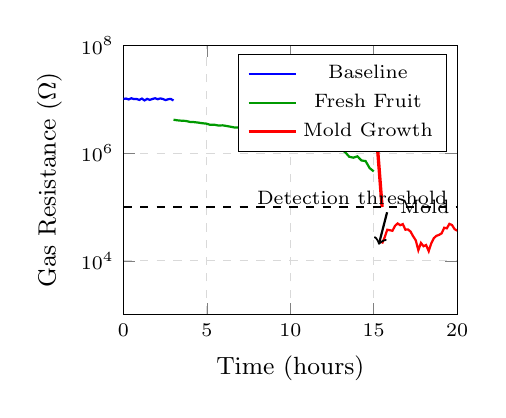
\begin{tikzpicture}
\begin{semilogyaxis}[
    width=0.48\textwidth,
    height=5cm,
    xlabel={Time (hours)},
    ylabel={Gas Resistance ($\Omega$)},
    xmin=0, xmax=20,
    ymin=1000, ymax=100000000,
    legend pos=north east,
    legend style={font=\scriptsize},
    grid=major,
    grid style={dashed, gray!30},
    tick label style={font=\scriptsize},
    label style={font=\small},
]

% Baseline phase (high resistance ~10M Ohm)
\addplot[blue, thick, domain=0:3, samples=20]
    {10000000 + 500000*rand};
\addlegendentry{Baseline}

% Fresh fruit phase (variable, 100k - 10M)
\addplot[green!60!black, thick, domain=3:15, samples=50]
    {5000000 - 300000*x + 100000*rand};
\addlegendentry{Fresh Fruit}

% Mold introduction - sharp drop
\addplot[red, very thick, domain=15:15.5, samples=10]
    {10^(7 - 4*(x-15))};

% Mold phase (low resistance 5k-50k)
\addplot[red, thick, domain=15.5:20, samples=30]
    {30000 + 15000*sin(deg(x*2)) + 5000*rand};
\addlegendentry{Mold Growth}

% Annotations
\node[font=\scriptsize, anchor=west] at (axis cs:16,100000) {Mold detected};
\draw[->, thick] (axis cs:15.8,80000) -- (axis cs:15.3,20000);

% Threshold line
\addplot[dashed, black, domain=0:20] {100000};
\node[font=\scriptsize, anchor=east] at (axis cs:20,150000) {Detection threshold};

\end{semilogyaxis}
\end{tikzpicture}
\caption{Gas resistance response during the spoilage experiment. The BME688 sensor shows a characteristic 3-order-of-magnitude drop from $\approx$10\,M$\Omega$ (clean air) to $\approx$5--50\,k$\Omega$ upon mold growth, providing a clear spoilage signature.}
\label{fig:gas_resistance}
\end{figure}

% Requires: \usepackage{pgfplots}

\begin{figure}[ht]
\centering
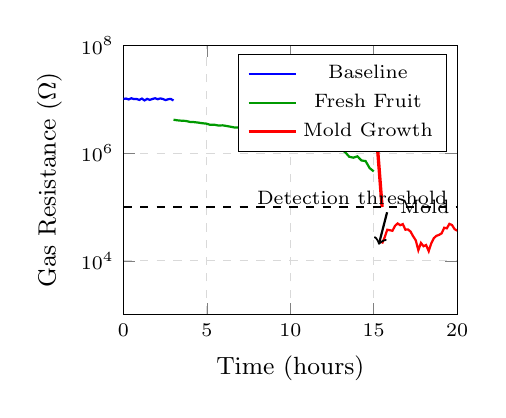
\begin{tikzpicture}
\begin{semilogyaxis}[
    width=0.48\textwidth,
    height=5cm,
    xlabel={Time (hours)},
    ylabel={Gas Resistance ($\Omega$)},
    xmin=0, xmax=20,
    ymin=1000, ymax=100000000,
    legend pos=north east,
    legend style={font=\scriptsize},
    grid=major,
    grid style={dashed, gray!30},
    tick label style={font=\scriptsize},
    label style={font=\small},
]

% Baseline phase (high resistance ~10M Ohm)
\addplot[blue, thick, domain=0:3, samples=20]
    {10000000 + 500000*rand};
\addlegendentry{Baseline}

% Fresh fruit phase (variable, 100k - 10M)
\addplot[green!60!black, thick, domain=3:15, samples=50]
    {5000000 - 300000*x + 100000*rand};
\addlegendentry{Fresh Fruit}

% Mold introduction - sharp drop
\addplot[red, very thick, domain=15:15.5, samples=10]
    {10^(7 - 4*(x-15))};

% Mold phase (low resistance 5k-50k)
\addplot[red, thick, domain=15.5:20, samples=30]
    {30000 + 15000*sin(deg(x*2)) + 5000*rand};
\addlegendentry{Mold Growth}

% Annotations
\node[font=\scriptsize, anchor=west] at (axis cs:16,100000) {Mold detected};
\draw[->, thick] (axis cs:15.8,80000) -- (axis cs:15.3,20000);

% Threshold line
\addplot[dashed, black, domain=0:20] {100000};
\node[font=\scriptsize, anchor=east] at (axis cs:20,150000) {Detection threshold};

\end{semilogyaxis}
\end{tikzpicture}
\caption{Gas resistance response during the spoilage experiment. The BME688 sensor shows a characteristic 3-order-of-magnitude drop from $\approx$10\,M$\Omega$ (clean air) to $\approx$5--50\,k$\Omega$ upon mold growth, providing a clear spoilage signature.}
\label{fig:gas_resistance}
\end{figure}

% Requires: \usepackage{pgfplots}

\begin{figure}[ht]
\centering
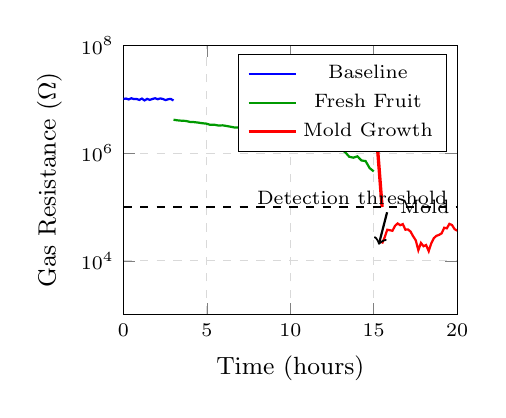
\begin{tikzpicture}
\begin{semilogyaxis}[
    width=0.48\textwidth,
    height=5cm,
    xlabel={Time (hours)},
    ylabel={Gas Resistance ($\Omega$)},
    xmin=0, xmax=20,
    ymin=1000, ymax=100000000,
    legend pos=north east,
    legend style={font=\scriptsize},
    grid=major,
    grid style={dashed, gray!30},
    tick label style={font=\scriptsize},
    label style={font=\small},
]

% Baseline phase (high resistance ~10M Ohm)
\addplot[blue, thick, domain=0:3, samples=20]
    {10000000 + 500000*rand};
\addlegendentry{Baseline}

% Fresh fruit phase (variable, 100k - 10M)
\addplot[green!60!black, thick, domain=3:15, samples=50]
    {5000000 - 300000*x + 100000*rand};
\addlegendentry{Fresh Fruit}

% Mold introduction - sharp drop
\addplot[red, very thick, domain=15:15.5, samples=10]
    {10^(7 - 4*(x-15))};

% Mold phase (low resistance 5k-50k)
\addplot[red, thick, domain=15.5:20, samples=30]
    {30000 + 15000*sin(deg(x*2)) + 5000*rand};
\addlegendentry{Mold Growth}

% Annotations
\node[font=\scriptsize, anchor=west] at (axis cs:16,100000) {Mold detected};
\draw[->, thick] (axis cs:15.8,80000) -- (axis cs:15.3,20000);

% Threshold line
\addplot[dashed, black, domain=0:20] {100000};
\node[font=\scriptsize, anchor=east] at (axis cs:20,150000) {Detection threshold};

\end{semilogyaxis}
\end{tikzpicture}
\caption{Gas resistance response during the spoilage experiment. The BME688 sensor shows a characteristic 3-order-of-magnitude drop from $\approx$10\,M$\Omega$ (clean air) to $\approx$5--50\,k$\Omega$ upon mold growth, providing a clear spoilage signature.}
\label{fig:gas_resistance}
\end{figure}

% Requires: \usepackage{pgfplots}

\begin{figure}[ht]
\centering
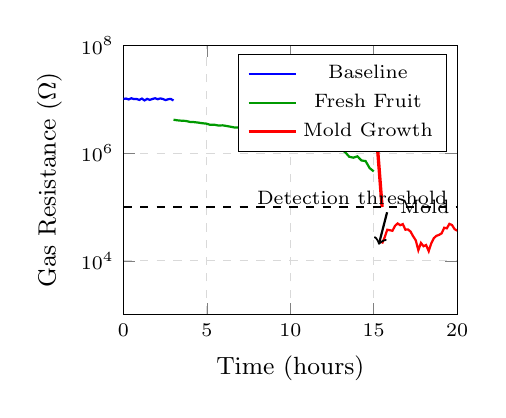
\begin{tikzpicture}
\begin{semilogyaxis}[
    width=0.48\textwidth,
    height=5cm,
    xlabel={Time (hours)},
    ylabel={Gas Resistance ($\Omega$)},
    xmin=0, xmax=20,
    ymin=1000, ymax=100000000,
    legend pos=north east,
    legend style={font=\scriptsize},
    grid=major,
    grid style={dashed, gray!30},
    tick label style={font=\scriptsize},
    label style={font=\small},
]

% Baseline phase (high resistance ~10M Ohm)
\addplot[blue, thick, domain=0:3, samples=20]
    {10000000 + 500000*rand};
\addlegendentry{Baseline}

% Fresh fruit phase (variable, 100k - 10M)
\addplot[green!60!black, thick, domain=3:15, samples=50]
    {5000000 - 300000*x + 100000*rand};
\addlegendentry{Fresh Fruit}

% Mold introduction - sharp drop
\addplot[red, very thick, domain=15:15.5, samples=10]
    {10^(7 - 4*(x-15))};

% Mold phase (low resistance 5k-50k)
\addplot[red, thick, domain=15.5:20, samples=30]
    {30000 + 15000*sin(deg(x*2)) + 5000*rand};
\addlegendentry{Mold Growth}

% Annotations
\node[font=\scriptsize, anchor=west] at (axis cs:16,100000) {Mold detected};
\draw[->, thick] (axis cs:15.8,80000) -- (axis cs:15.3,20000);

% Threshold line
\addplot[dashed, black, domain=0:20] {100000};
\node[font=\scriptsize, anchor=east] at (axis cs:20,150000) {Detection threshold};

\end{semilogyaxis}
\end{tikzpicture}
\caption{Gas resistance response during the spoilage experiment. The BME688 sensor shows a characteristic 3-order-of-magnitude drop from $\approx$10\,M$\Omega$ (clean air) to $\approx$5--50\,k$\Omega$ upon mold growth, providing a clear spoilage signature.}
\label{fig:gas_resistance}
\end{figure}
